%%%%%%%%%%%%%%%%%%%%%%%%%%%%%%%%%%%%%%%%%%%%%%%%%%%%%%%%%%%%%%%%%%%%%%%%%%%%%% 
\section {Reconstruction and background rejection}

Discuss reconstruction, selection, and rejection cuts

\begin{figure}
  \centering
  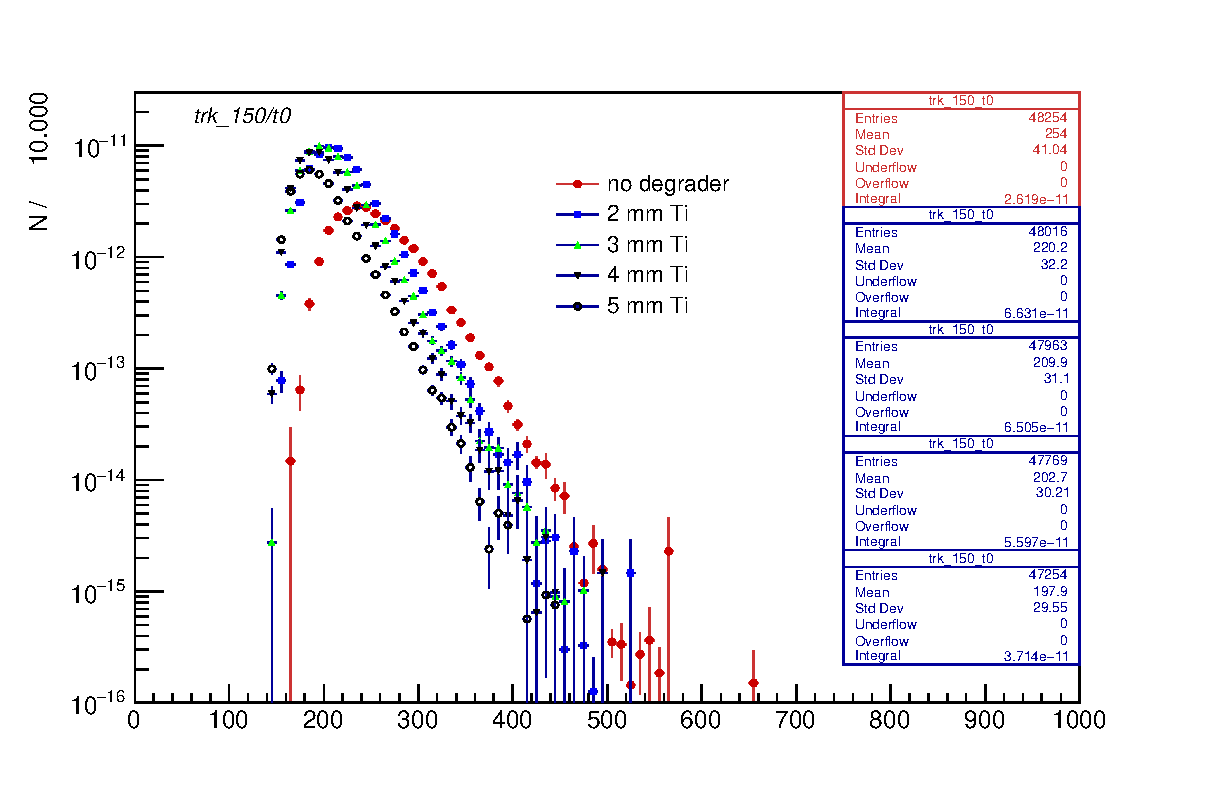
\includegraphics[width = 0.99\linewidth]{pdf/figure_00001}
  \caption{
    \label{fig:pions_timing}
    Distributions of the reconstructed $\pi^+ \to e^+ \nu$ track time for different degrader thicknesses
  }
\end{figure}



%%%%%%%%%%%%%%%%%%%%%%%%%%%%%%%%%%%%%%%%%%%%%%%%%%%%%%%%%%%%%%%%%%%%%%%%%%%%%%
\subsection{Track selection cuts}

Give a table of initial track selection cuts - close to ``Set C''...

\begin{figure}[H]
  % \centering
  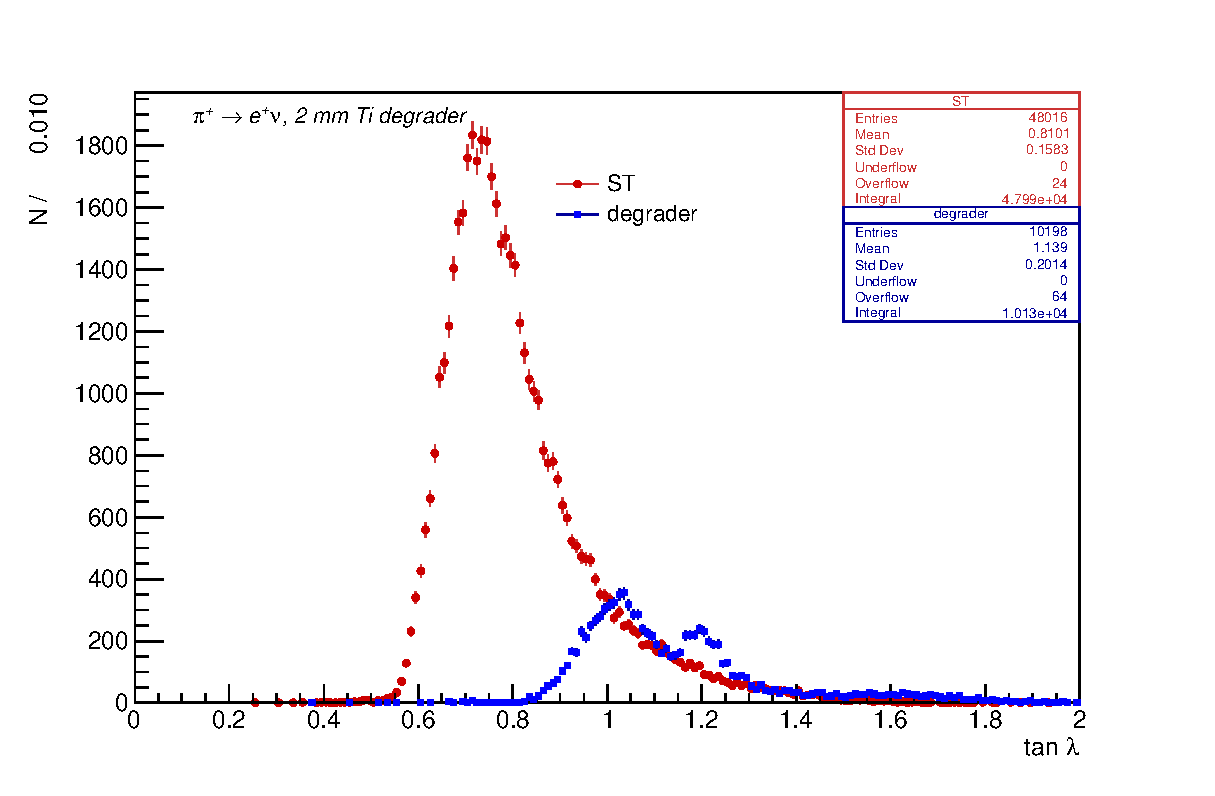
\includegraphics[width=0.55\linewidth]{pdf/figure_00203}
  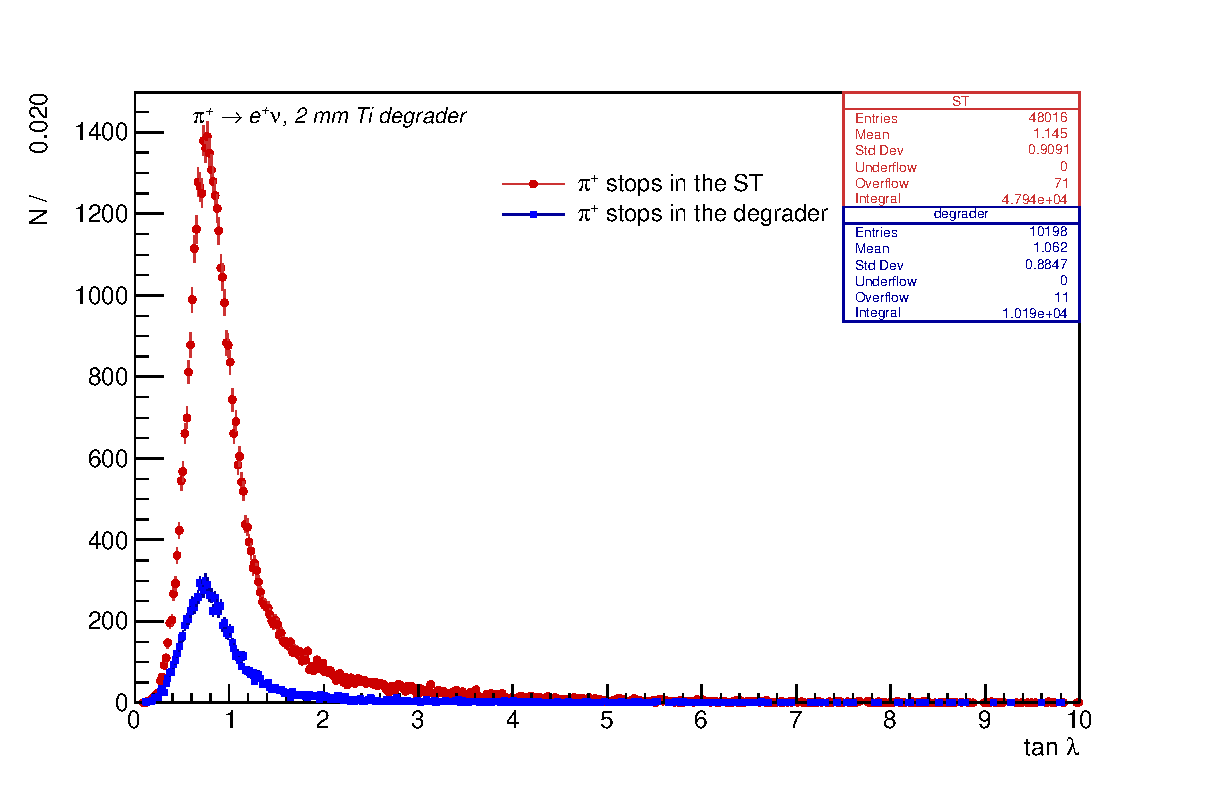
\includegraphics[width=0.55\linewidth]{pdf/figure_00204}
  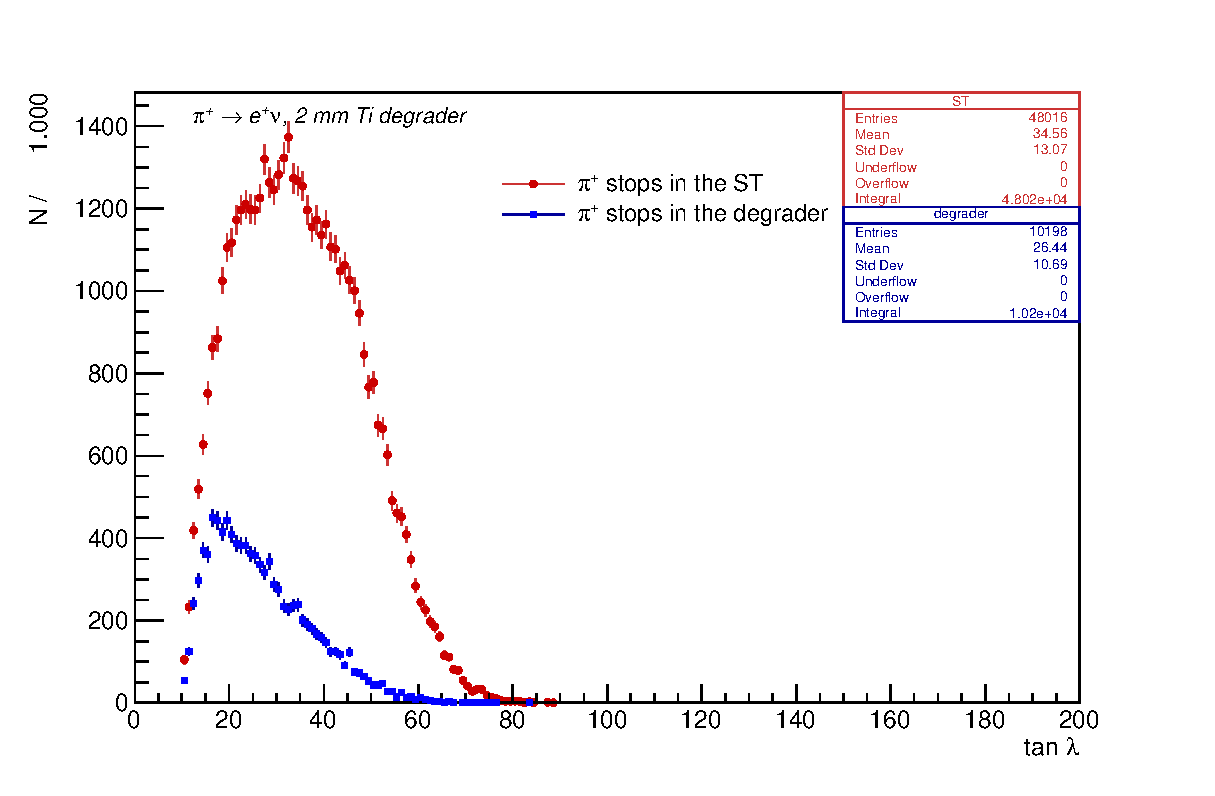
\includegraphics[width=0.55\linewidth]{pdf/figure_00205}
  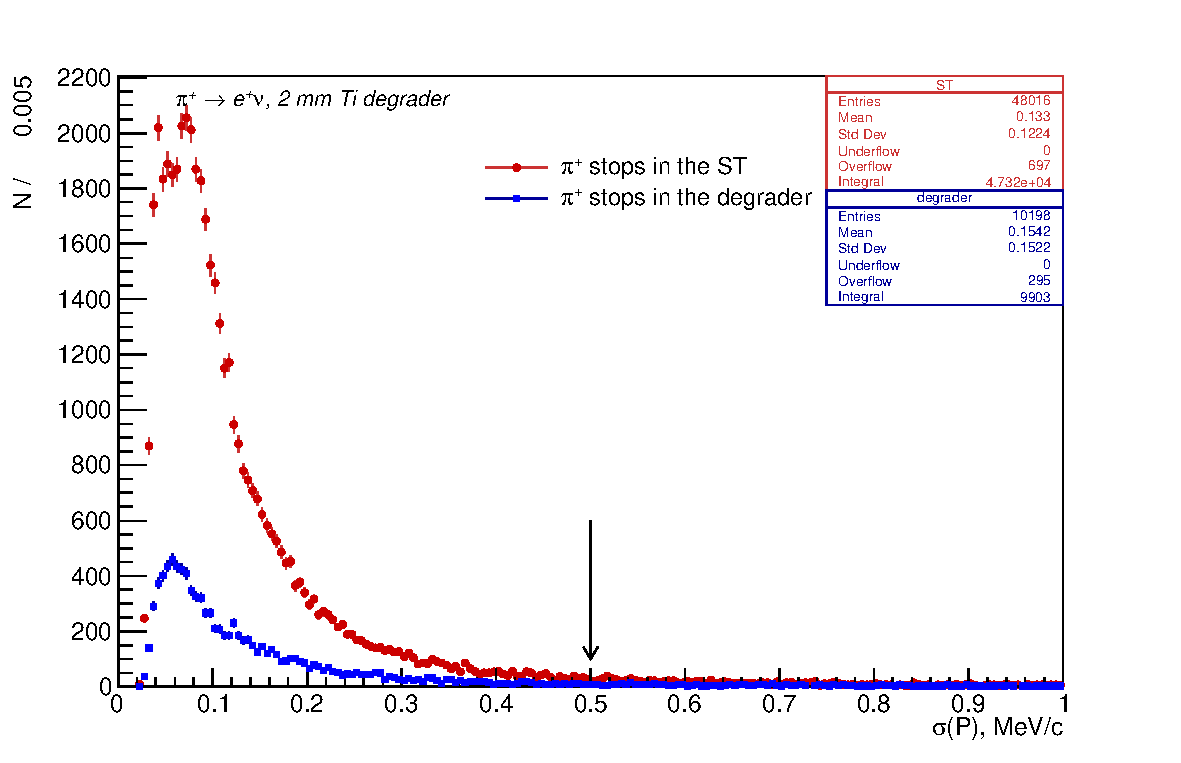
\includegraphics[width=0.55\linewidth]{pdf/figure_00206}
  \caption{
    % \label{fig:deg_vs_no_degrader_time}
    Distributions of the track ID variables 
  }
\end{figure}

{\red probably need ``N-1'' plots here}

%%%%%%%%%%%%%%%%%%%%%%%%%%%%%%%%%%%%%%%%%%%%%%%%%%%%%%%%%%%%%%%%%%%%%%%%%%%%%%
\subsection{Signal and signal reconstruction efficiency}


%%%%%%%%%%%%%%%%%%%%%%%%%%%%%%%%%%%%%%%%%%%%%%%%%%%%%%%%%%%%%%%%%%%%%%%%%%%%%%
\subsection{Decays of pions stopped in degrader}

\begin{figure}[H]
  % \centering
  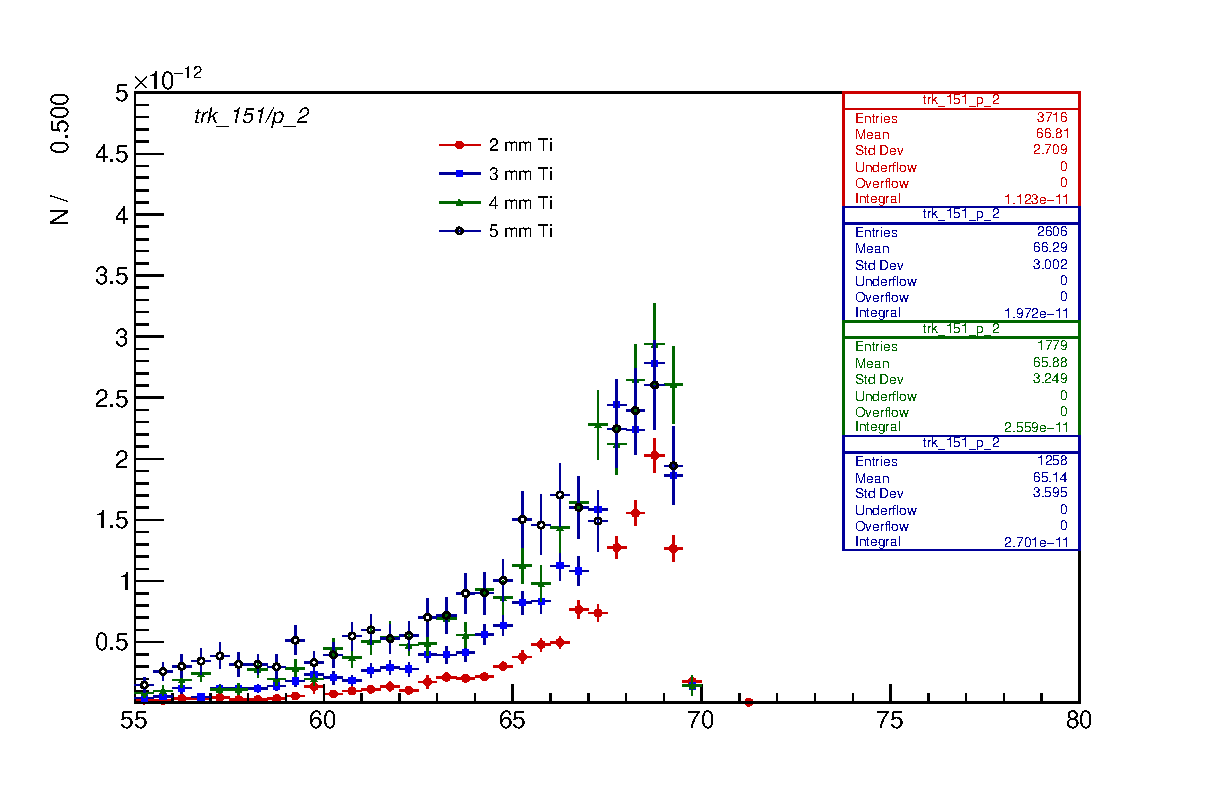
\includegraphics[width=0.55\linewidth]{pdf/figure_00011}
  \caption{
    % \label{fig:deg_vs_no_degrader_time}
  }
\end{figure}

\begin{figure}[H]
  % \centering
  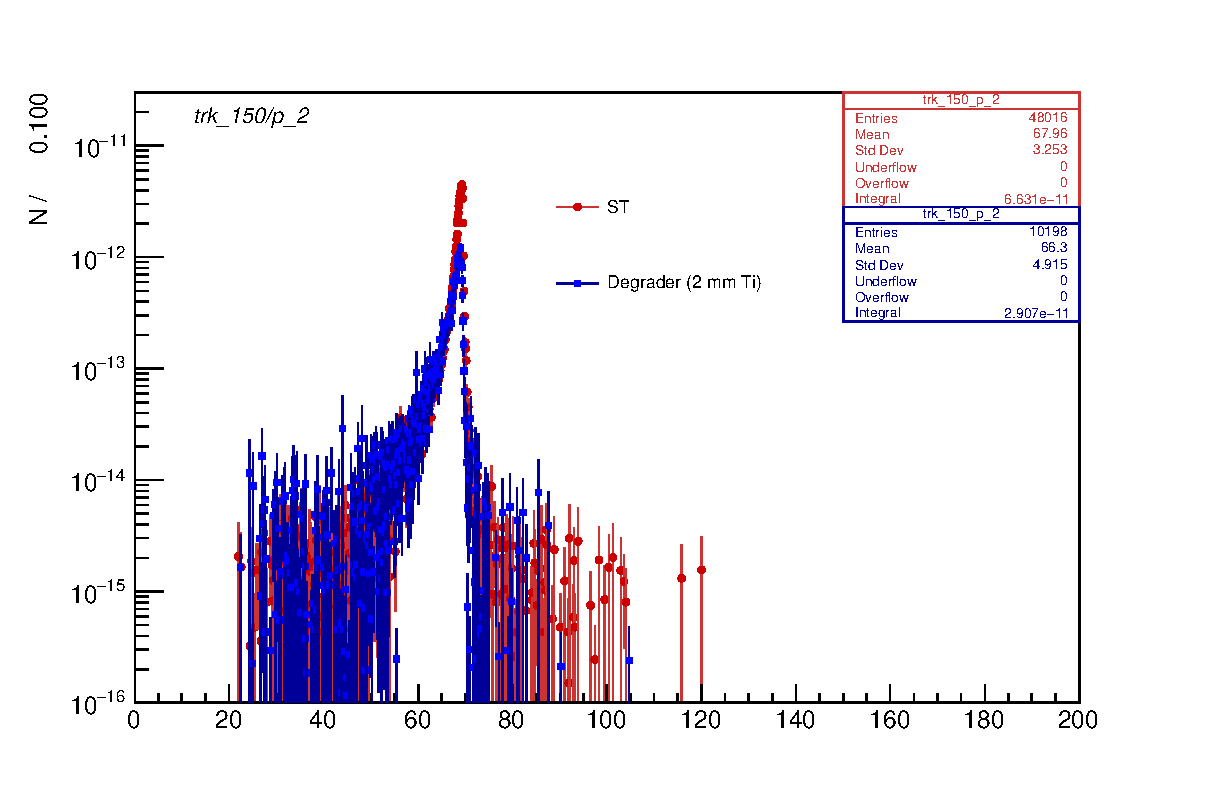
\includegraphics[width=0.55\linewidth]{pdf/figure_00201}
  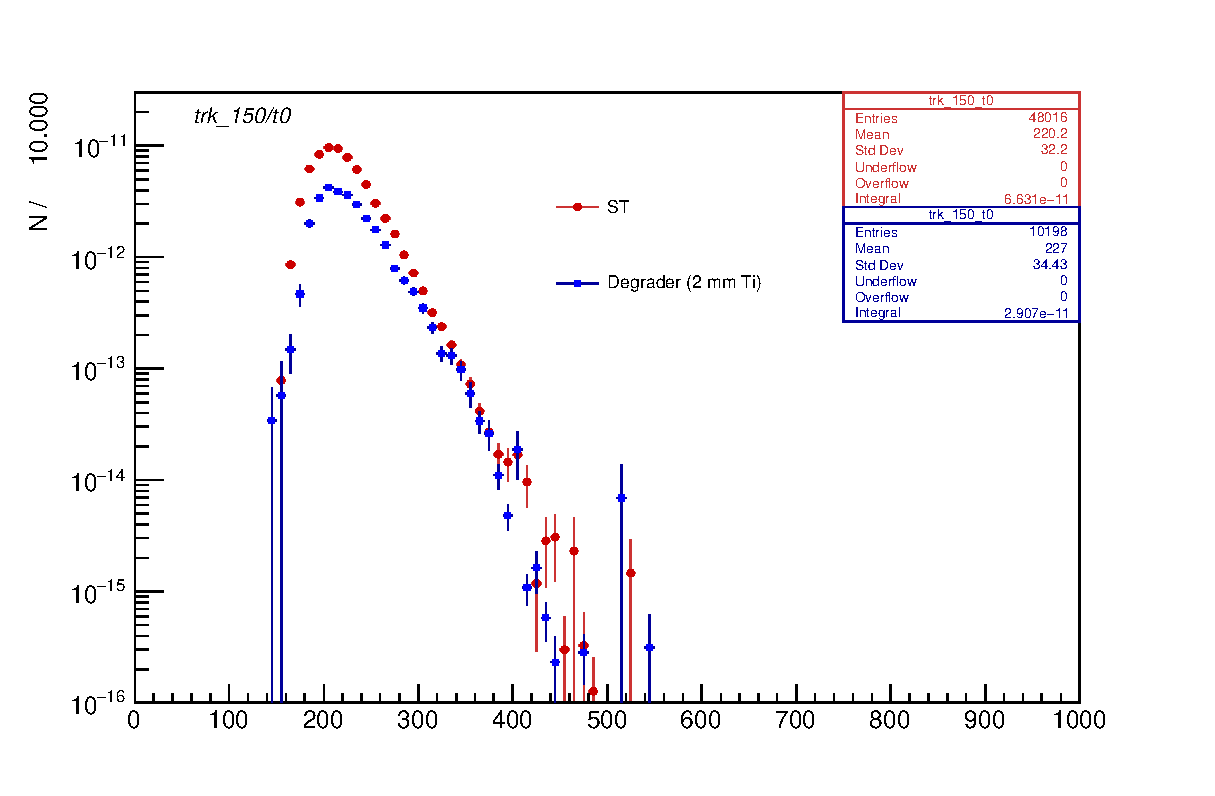
\includegraphics[width=0.55\linewidth]{pdf/figure_00202}
  \caption{
    % \label{fig:deg_vs_no_degrader_time}
  }
\end{figure}

\begin{figure}[H]
  % \centering
  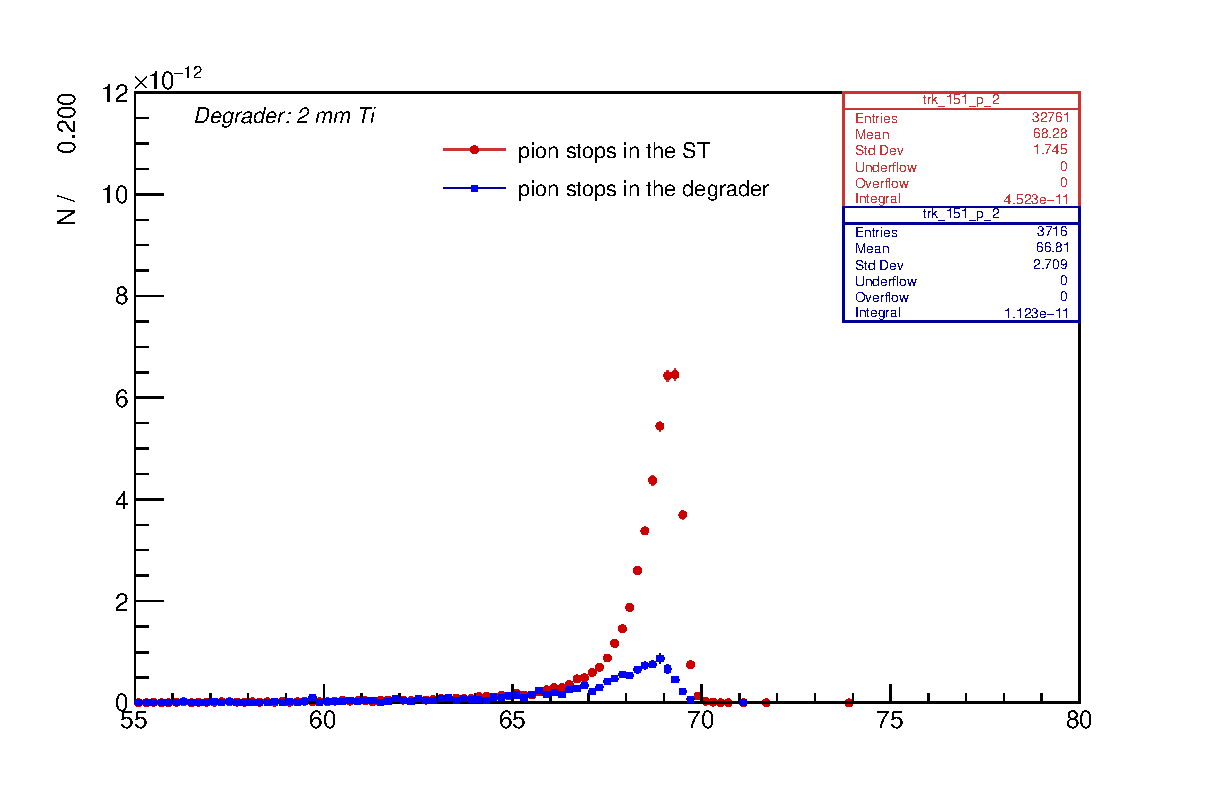
\includegraphics[width=0.55\linewidth]{pdf/figure_00211}
  \caption{
    % \label{fig:deg_vs_no_degrader_time}
  }
\end{figure}

\begin{figure}[H]
  % \centering
  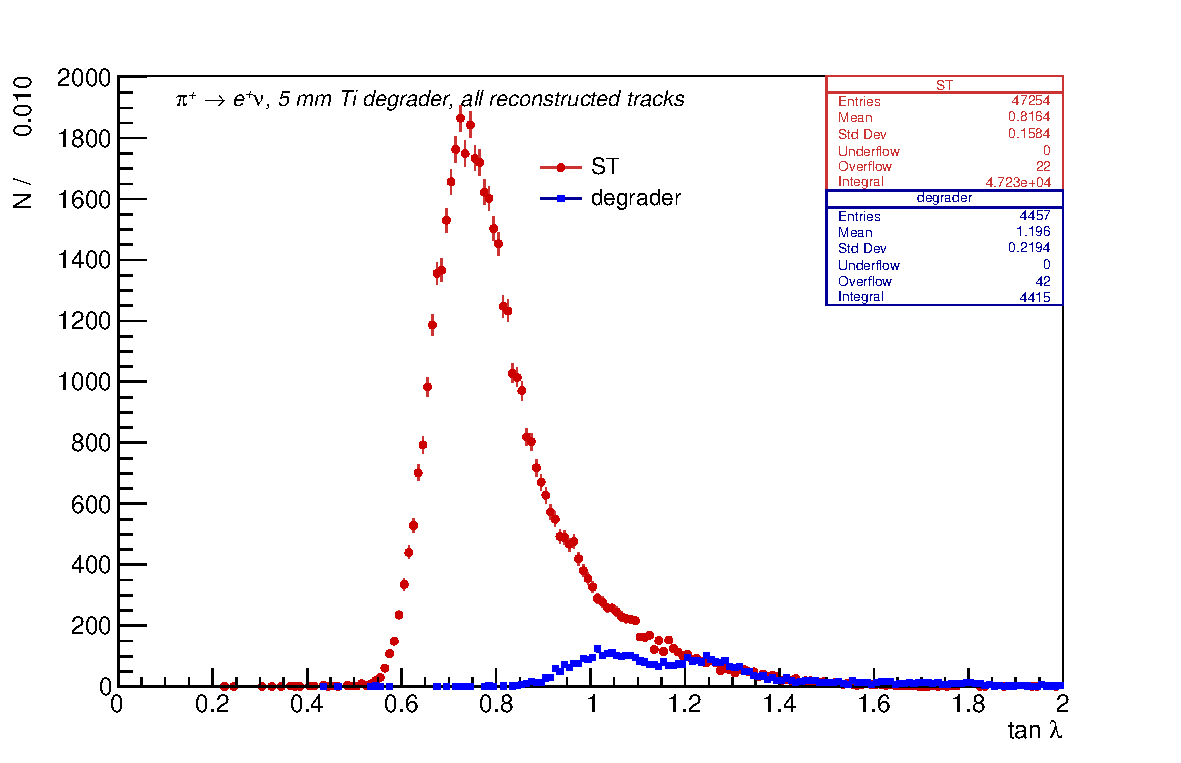
\includegraphics[width=0.55\linewidth]{pdf/figure_00503}
  \caption{
    % \label{fig:deg_vs_no_degrader_time}
    track ID variables, 5 mm Ti degrader, all reconstructed tracks
  }
\end{figure}

\begin{figure}[H]
  % \centering
  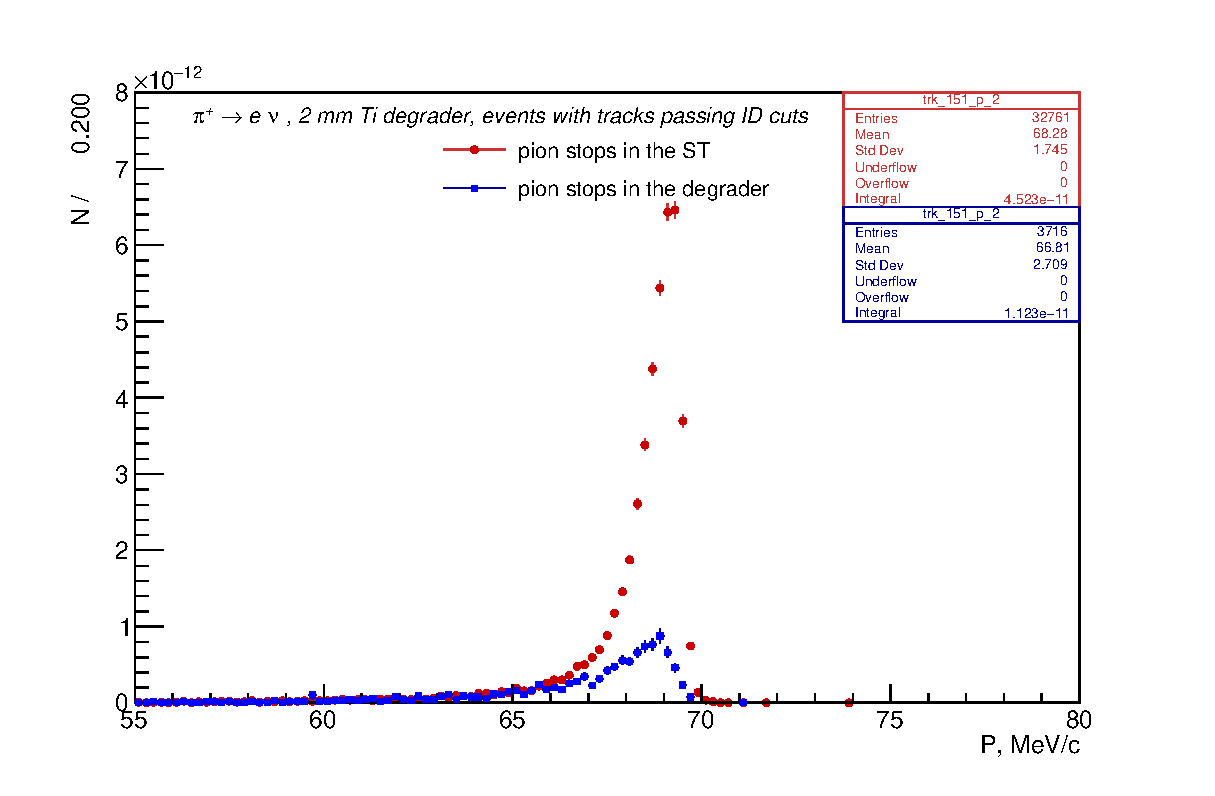
\includegraphics[width=0.55\linewidth]{pdf/figure_00261}
  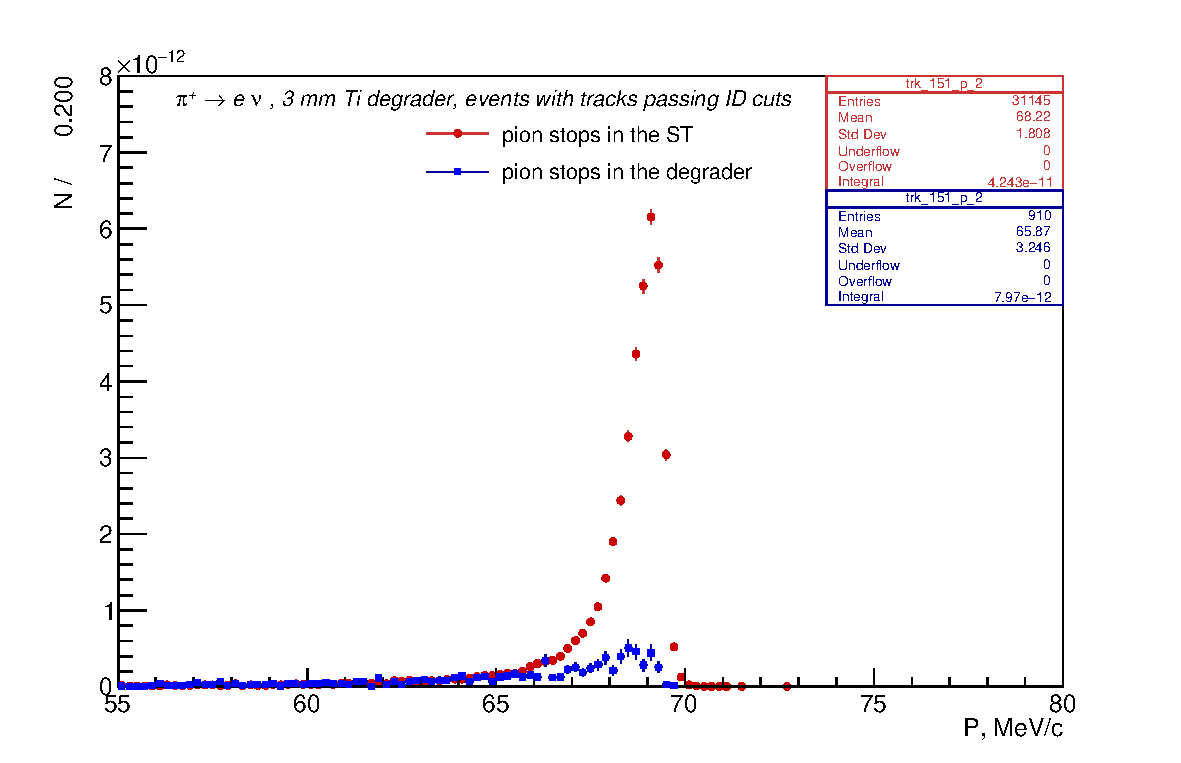
\includegraphics[width=0.55\linewidth]{pdf/figure_00361}
  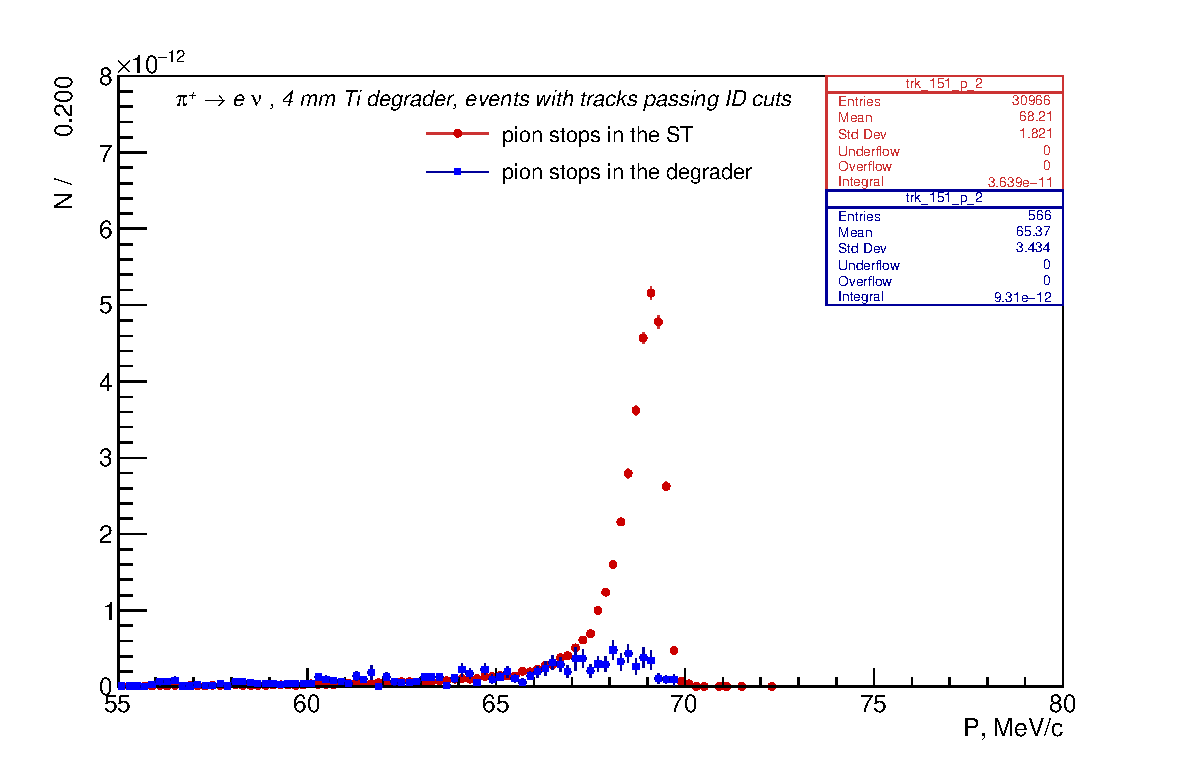
\includegraphics[width=0.55\linewidth]{pdf/figure_00461}
  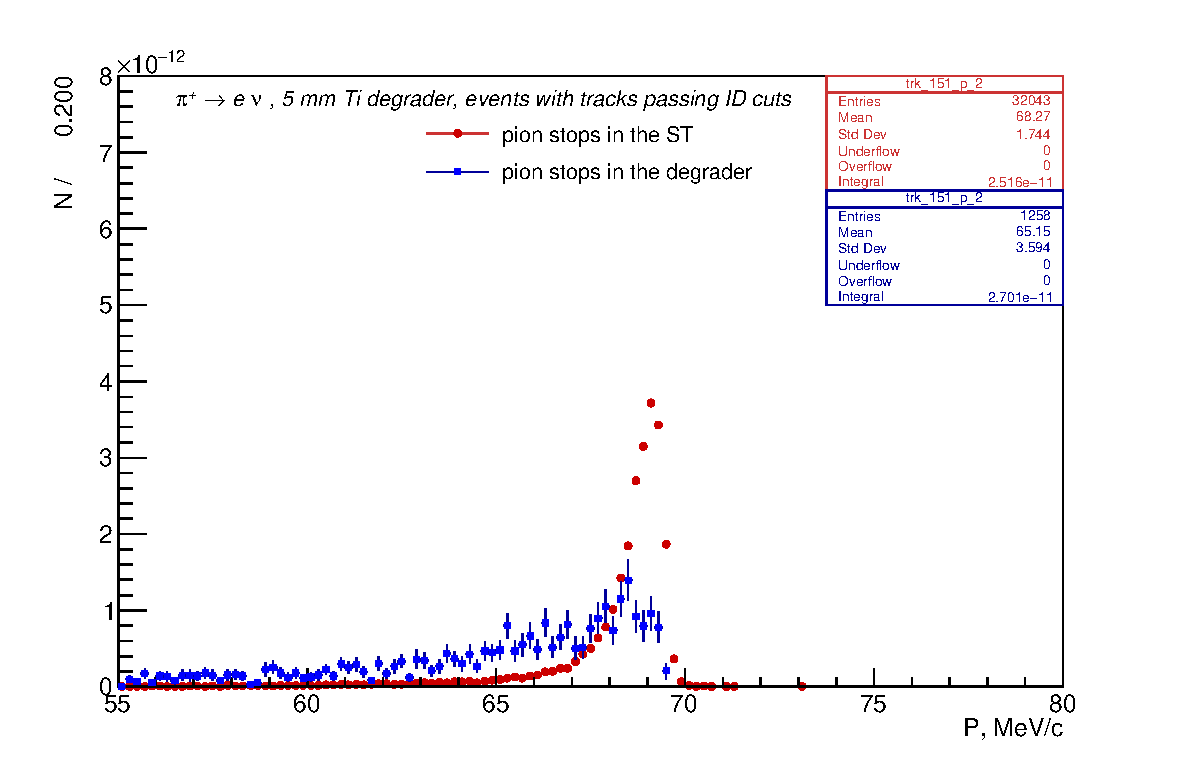
\includegraphics[width=0.55\linewidth]{pdf/figure_00561}
  \caption{
    % \label{fig:deg_vs_no_degrader_time}
    reconstructed e+ yield/POT for different degrader thicknesses.
    ST vs DEG
  }
\end{figure}


%%%%%%%%%%%%%%%%%%%%%%%%%%%%%%%%%%%%%%%%%%%%%%%%%%%%%%%%%%%%%%%%%%%%%%%%%%%%%%
\section{Signal selection efficiency}

{\red
  \begin{itemize}
  \item 
    put N-1 plots here, an efficiency table
  \item
    quote total selection efficiency for pienu decays in the ST
  \end{itemize}
}

\begin{figure}[H]
  % \centering
  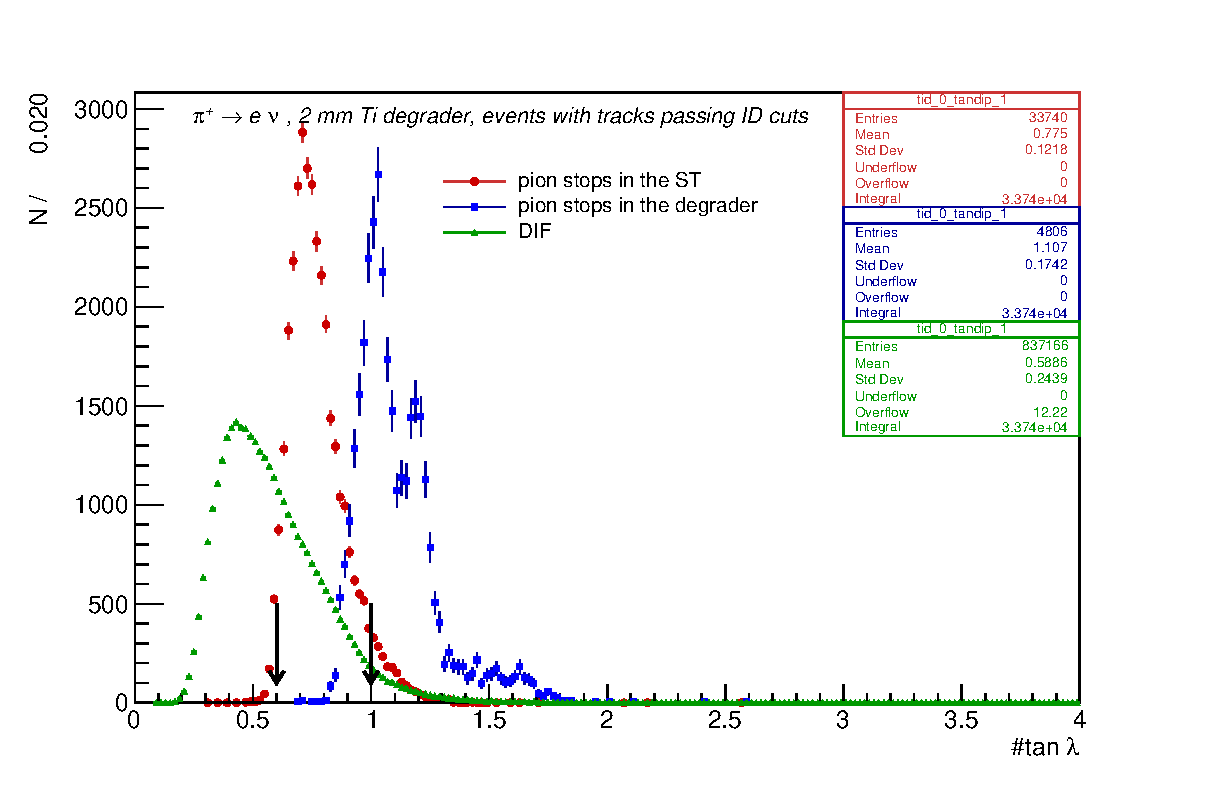
\includegraphics[width=0.55\linewidth]{pdf/figure_00273}
  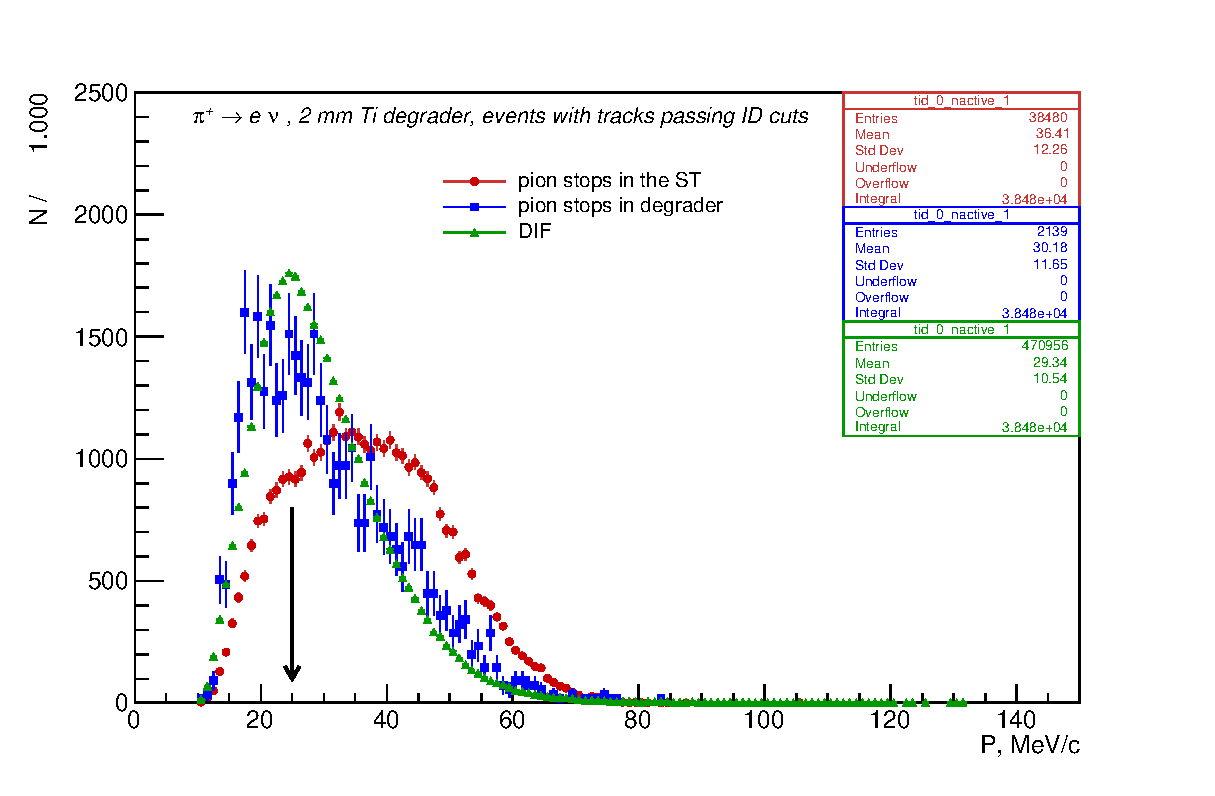
\includegraphics[width=0.55\linewidth]{pdf/figure_00274}
  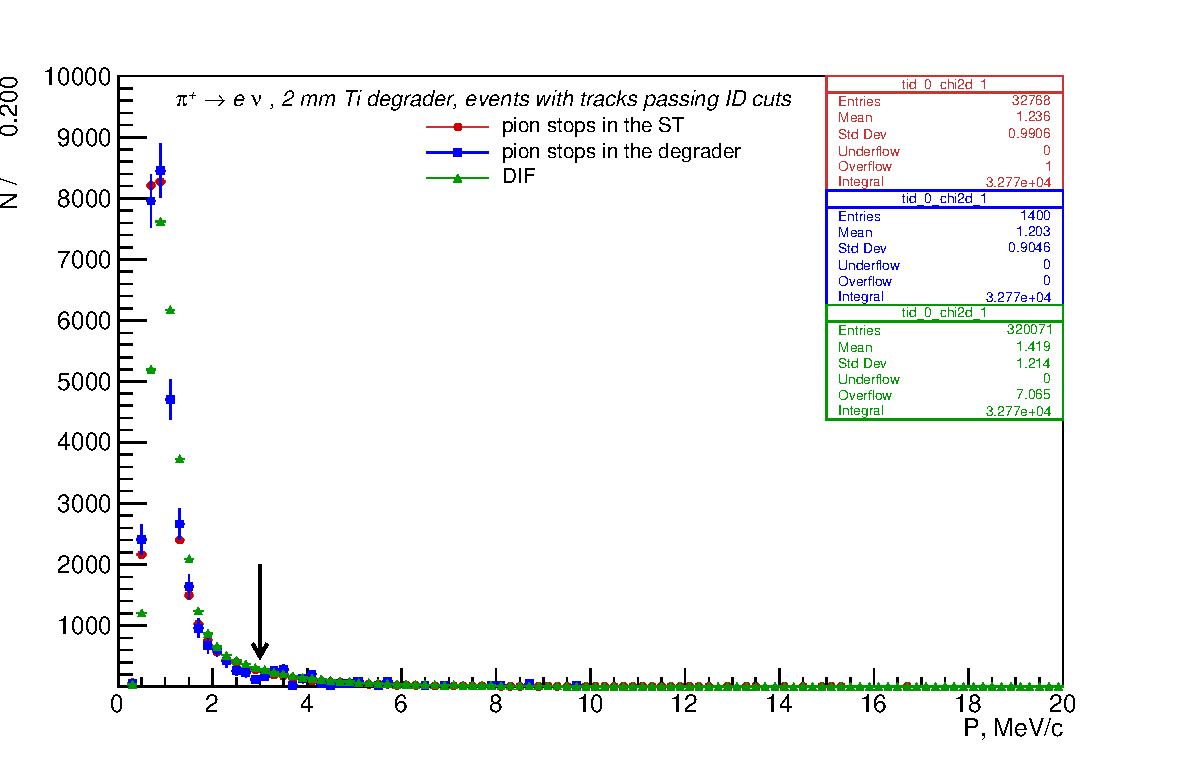
\includegraphics[width=0.55\linewidth]{pdf/figure_00275}
  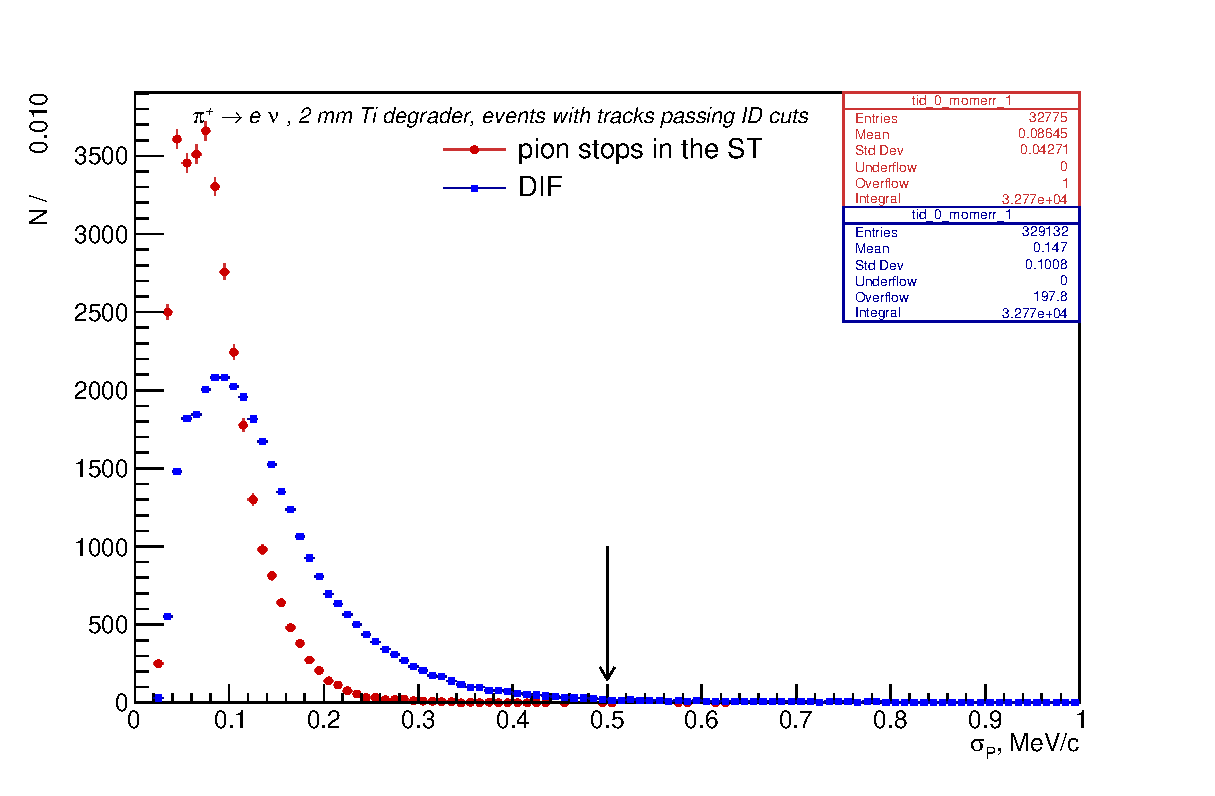
\includegraphics[width=0.55\linewidth]{pdf/figure_00276}
  \caption{
    % \label{fig:deg_vs_no_degrader_time}
    distributions of ID variables after ``N-1'' cuts
  }
\end{figure}


%%%%%%%%%%%%%%%%%%%%%%%%%%%%%%%%%%%%%%%%%%%%%%%%%%%%%%%%%%%%%%%%%%%%%%%%%%%%%%
\subsection {Signal Yields for different degrader thicknesses}
\begin{figure}[H]
  % \centering
  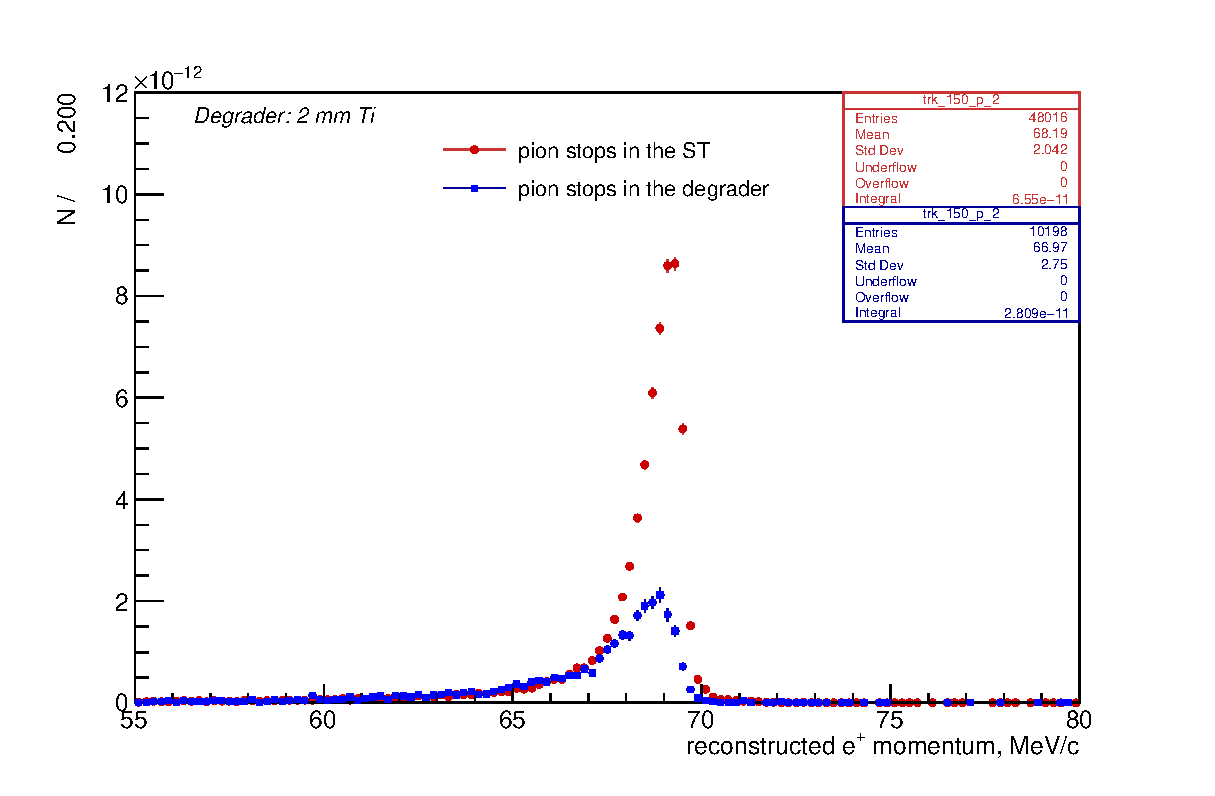
\includegraphics[width=0.55\linewidth]{pdf/figure_00251}
  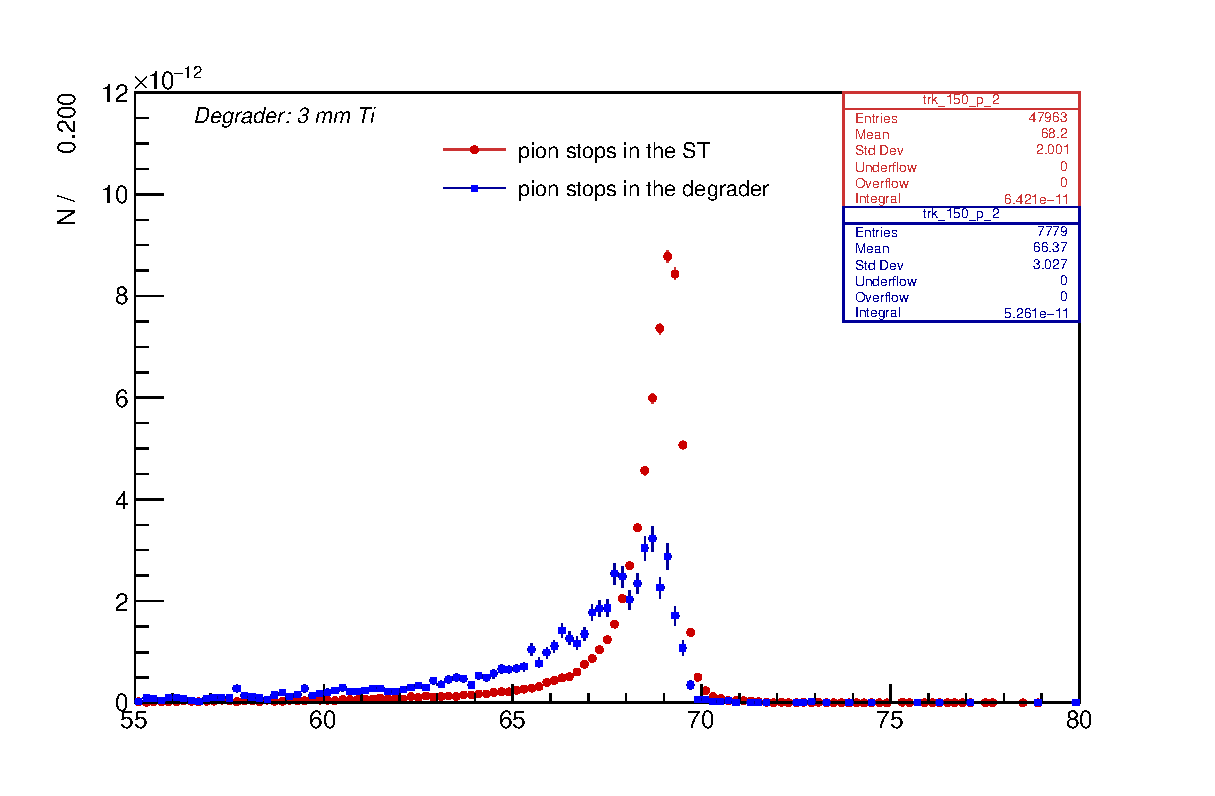
\includegraphics[width=0.55\linewidth]{pdf/figure_00351}
  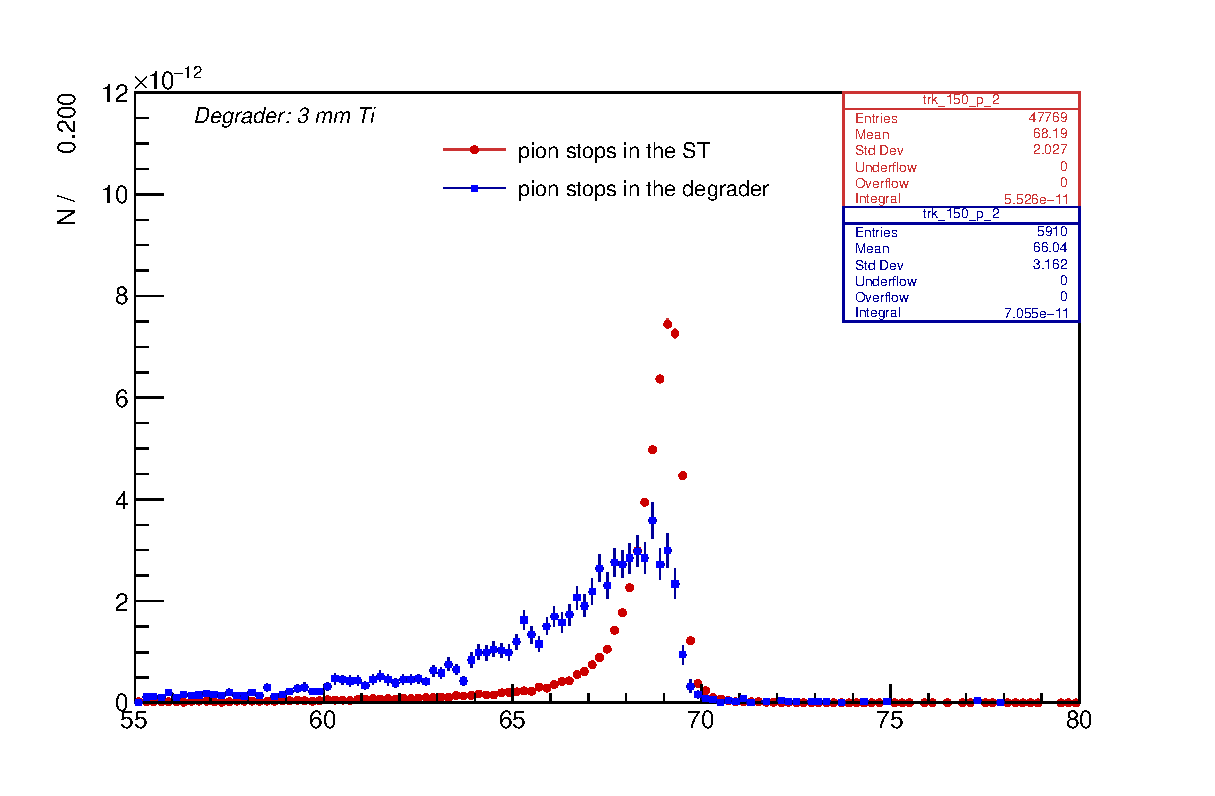
\includegraphics[width=0.55\linewidth]{pdf/figure_00451}
  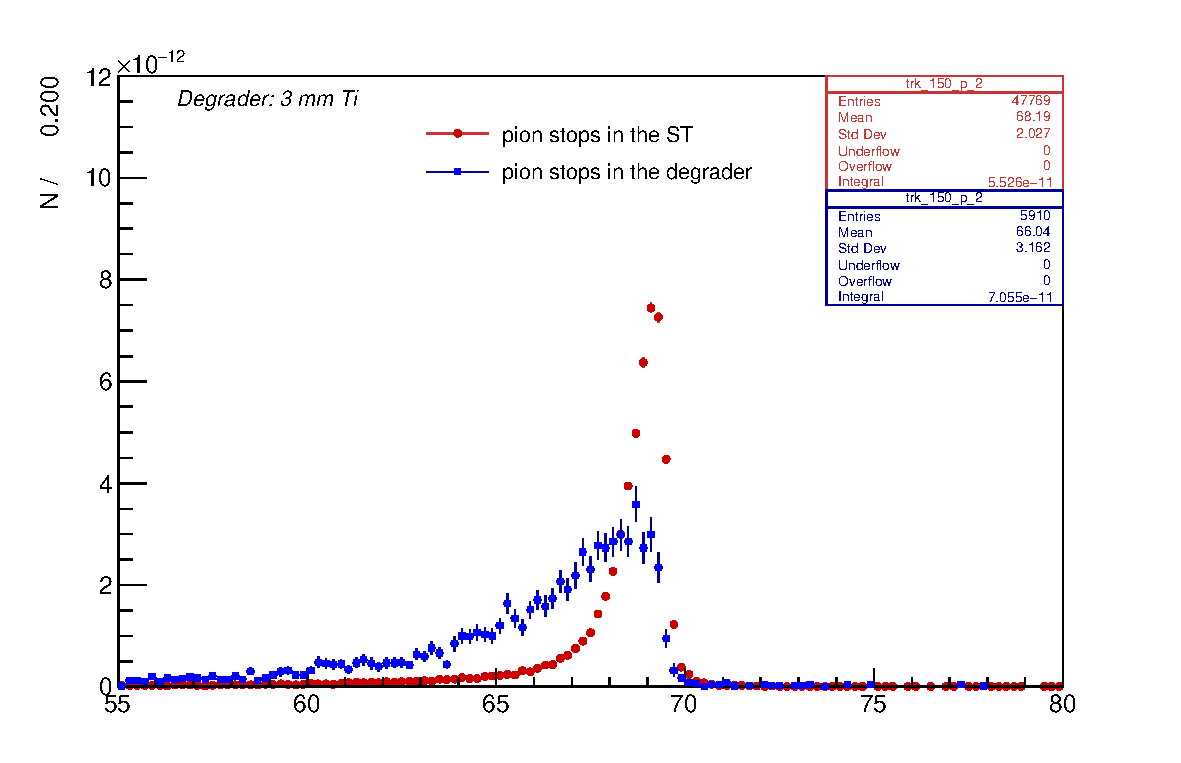
\includegraphics[width=0.55\linewidth]{pdf/figure_00551}
  \caption{
    % \label{fig:deg_vs_no_degrader_time}
  }
\end{figure}

{\red need the same plots after the track selection cuts}

%%%%%%%%%%%%%%%%%%%%%%%%%%%%%%%%%%%%%%%%%%%%%%%%%%%%%%%%%%%%%%%%%%%%%%%%%%%%%%
\subsection{Initial selection - results}




%%%%%%%%%%%%%%%%%%%%%%%%%%%%%%%%%%%%%%%%%%%%%%%%%%%%%%%%%%%%%%%%%%%%%%%%%%%%%%
\subsection{Removing muon decays in the tracker}

One of the most dangerous topologies comes from the muon decays in flight backwards in the tracker,
so a positron is produced upstream with small pZ.

In case the pattern recognition uses hits in every second station, the positrons can be misreconstructed
as particles with higher momentum.

In this case the number of hits in the time cluster is expected to be significantly higher
than the number of hits reconstructed on the track.

%%%%%%%%%%%%%%%%%%%%%%%%%%%%%%%%%%%%%%%%%%%%%%%%%%%%%%%%%%%%%%%%%%%%%%%%%%%%%%
\subsection{Tight selection - results}


\begin{figure}[H]
  % \centering
  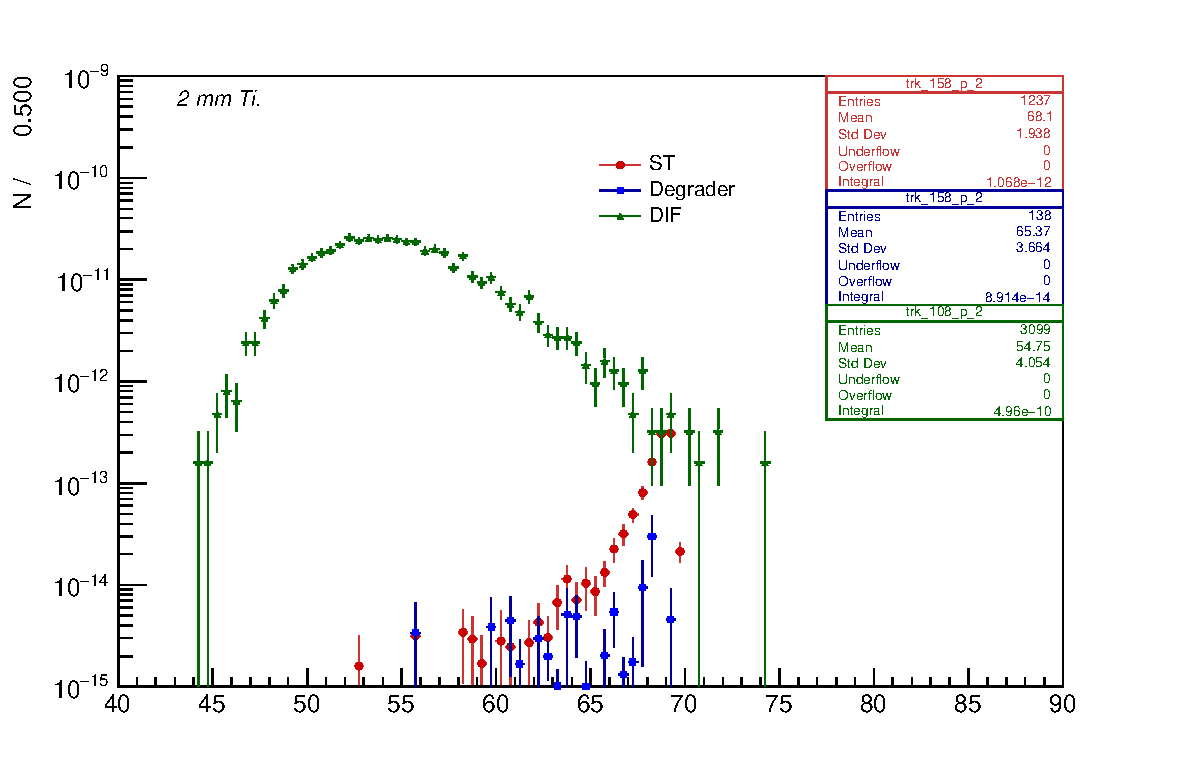
\includegraphics[width=0.55\linewidth]{pdf/figure_00231}
  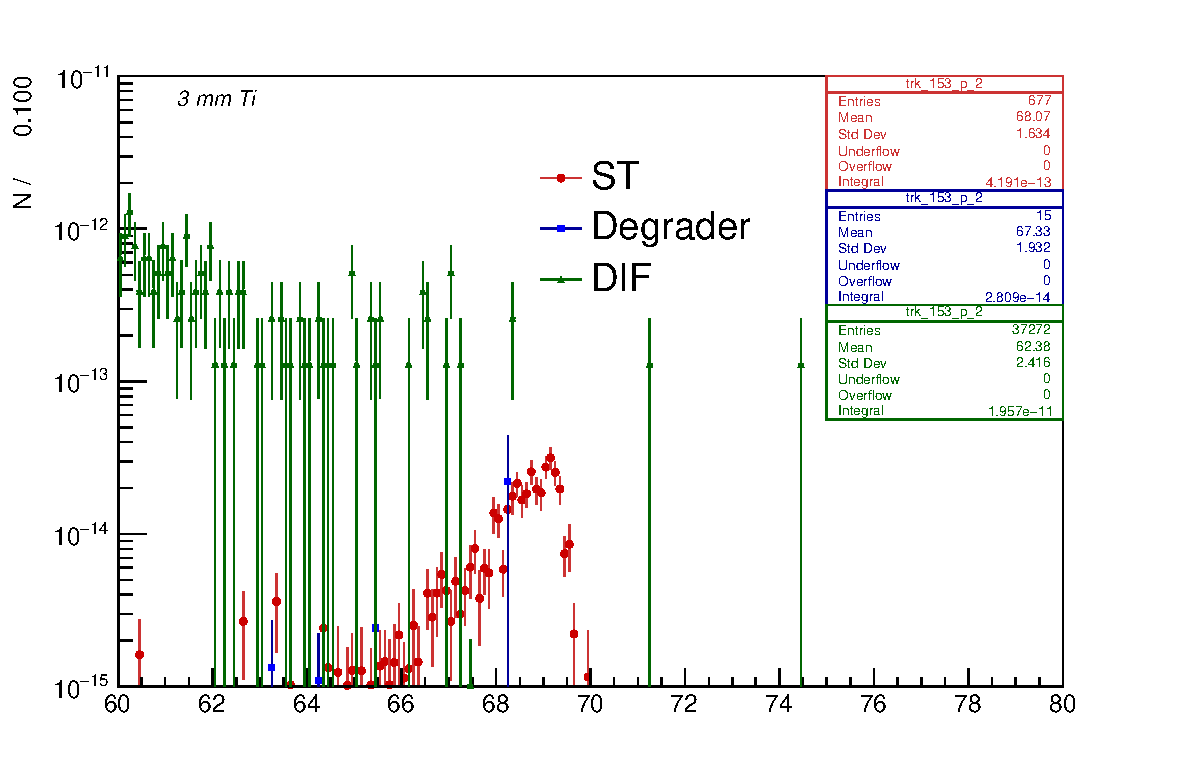
\includegraphics[width=0.55\linewidth]{pdf/figure_00331}
  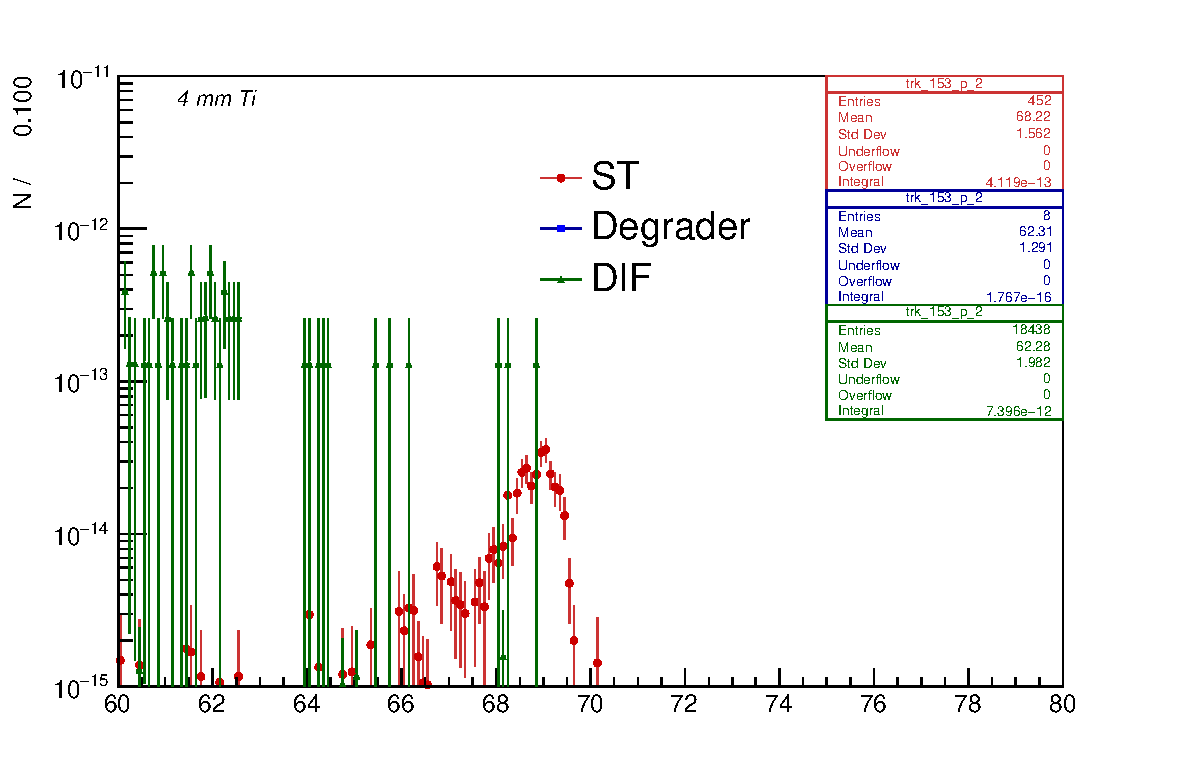
\includegraphics[width=0.55\linewidth]{pdf/figure_00431}
  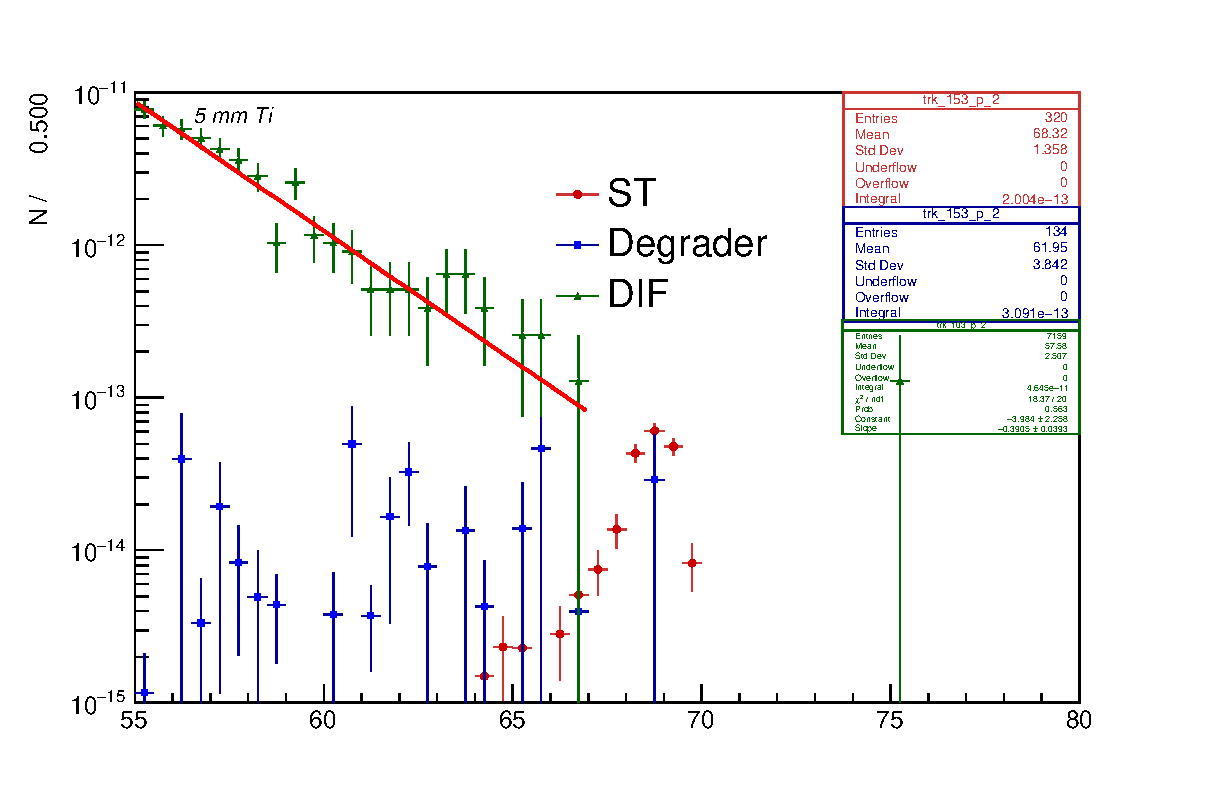
\includegraphics[width=0.55\linewidth]{pdf/figure_00531}
  \caption{
    \label{fig:deg_3mm_mom}
  }
\end{figure}

For degrader thickness of 4mm, a visual scan of DIF events above 65 MeV/c surviving
the tight selection cuts has been performed.

All surviving events represent an irreducible background and can't be rejected.

%%% Local Variables:
%%% mode: latex
%%% TeX-master: "mu2e-xxxxx"
%%% End:
